\hthree{Agiles Projektmanagement}

\hfour{Grundlegendes}

Grundlegend kann gesagt werden, dass beim agilen Projektmanagement das gesamte Team in den Bereichen Umfang, Zeit und Kosten über eine hohe Flexibilität verfügt. Außerdem wird der Kunde in den gesamten Prozess des Projekts miteinbezogen und immer auf dem Laufenden gehalten, in welchem Stand sich das Projekt befindet. Der Fokus liegt beim agilen Projektmanagement sehr stark auf dem Endprodukt und nicht auf Prozesse, welche im Vorhinein fix und starr definiert werden müssen. Also das Einhalten von Terminen, Kosten oder eines fixen Arbeitsaufwands wird eher oder ganz vernachlässigt. \cite{agil}

Dieses Dynamische und diese Flexibilität wird durch das "agil" zum Ausdruck gebracht. Änderungen im Ablauf des Projekts können unkompliziert eingearbeitet werden. Hierbei spricht man von sogenannten "Änderungsanträgen". Ein Änderungsantrag kann zum Beispiel einen der folgenden Punkte enthalten: \cite{agil}

\begin{itemize}
    \item Verbesserungen für das Produkt
    \item Eine Terminverschiebung
    \item Eine Erweiterung des Projektteams
    \item Die Reduzierung von Kosten für das Projekt
\end{itemize}

\cite{Aenderung}

Die Bedeutung von "Agil" hebt auch insbesondere die Vorteile von geringer Planungssicherheit hervor und besetzt diese positiv. \cite{agil} 

\hfour{Anwendungsgebiete}

Die Verwendung von agilem Projektmanagement bringt entscheidende Vorteile mit sich, wenn das Projekt:

\begin{itemize}
    \item keine klaren und deutlich definierten Anforderungen hat.
    \item vielen und ständigen Veränderungen in der Planung ausgesetzt ist.
    \item komplexere Ziele hat.
    \item kein deutliches Endziel hat oder kein vordefiniertes Endprodukt ist.
    \item schnelle Ergebnisse liefern muss und keine Zeit für langwierige Planung bleibt.
\end{itemize}

\cite{AnwendungAgil}

\hfour{Scrum}

\hfive{Allgemeines}

Das "Scrum Framework" wurde in den 1990ern von den beiden Softwareentwicklern Ken Schwaber und Jeff Sutherland entwickelt und veröffentlicht. 1995 wurde dann ein erstes Buch rund um "Scrum" von den beiden Entwicklern veröffentlicht. Diese Methode entwickelte sich über die Laufe der Jahre weiter und 2010 kam schließlich der erste "Scrum Guide" heraus. In diesem Guide definierten Schwaber und Sutherland "Scrum" folgendermaßen:

"Ein Rahmenwerk, mit dessen Hilfe Menschen komplexe adaptive Aufgabenstellungen angehen können, und durch das sie in die Lage versetzt werden, produktiv und kreativ Produkte mit dem höchstmöglichen Wert auszuliefern." \cite{Scrum}

Dieser "Scrum Guide" wurde von Ken Schwaber und Jeff Sutherland über Jahr gepflegt, erweitert und überarbeitet und ist in mehreren Sprachen zum Download aus dem Internet verfügbar. \cite{Scrum}

Der gewisse Grundgedanke hinter Scrum war die Entwicklung technischer Produkte wie mechatronische Produkte, aber auch Software. Die Idee in der Entwicklung agiler zu sein kam daher, dass ein Projekt (gerade in der Softwarebranche) nicht zu Beginn vom Anfang bis zum Ende in der benötigten Genauigkeit durchgeplant werden kann. Deshalb wurde "Scrum" als eine agile Entwicklungsmethode für technische Projekte entwickelt und eingeführt. \cite{Scrum}

\begin{figure}[H]
    \centering
    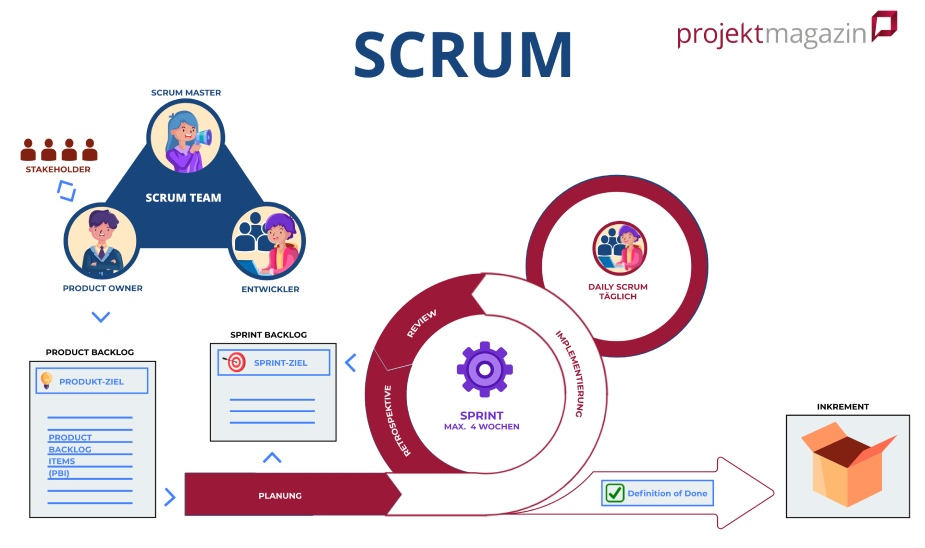
\includegraphics[width=\textwidth]{media/ProjectManagement/Scrum.jpg}
    \caption{Ablauf und Rollen in "Scrum" \cite{Scrum}}
\end{figure}

\hfive{Rollen in Scrum}

In "Scrum" gibt es drei unterschiedliche Rollen, welche im Ablauf des Projekts oder der Entwicklung für unterschiedliche Aufgaben- und Verantwortungsbereiche zuständig sind.

\begin{itemize}
    \item "Scrum Master"
    \item "Product Owner"
    \item Entwicklungsteam
\end{itemize}

\cite{Scrum}

\underline{"Scrum Master"}

Der "Scrum Master" ist die Rolle im Projekt, welche dafür verantwortlich ist, dass alle Beteiligten die Theorie und den Mechanismus hinter "Scrum" verstanden haben und die Fähigkeiten besitzen das Projekt nach "Scrum-Richtlinien" abzuwickeln. Im "Scrum Guide" wird die Funktion des "Scrum Master" wie folgt beschrieben: \cite{ScrumMaster}

"true leader who serves the Scrum Team and the larger organization" \cite{ScrumMaster}

Bricht man diesen Teil des Satzes nun auf konkrete Aufgaben- und Zuständigkeitsbereiche herunter kommen folgende Tätigkeiten in der Rolle des "Scrum Master" zustande:

\begin{itemize}
    \item "Er unterstützt den Product Owner beim Management des Product Backlogs." \cite{ScrumMaster}
    \item "Er moderiert die in Scrum vorgesehenen Arbeitstreffen." \cite{ScrumMaster}
    \item "Er unterstützt das Entwicklungsteam dabei, sich selbst zu organisieren und effizient zu arbeiten." \cite{ScrumMaster}
    \item "Er übernimmt die Kommunikation mit der Trägerorganisation, in der das Scrum Team eingebunden ist." \cite{ScrumMaster}
    \item "Er bemüht sich darum, Hemmnisse zu beseitigen, die den Arbeitsfortschritt behindern." \cite{ScrumMaster}
    \item "Er unterstützt die Trägerorganisation bei der Einführung von Scrum." \cite{ScrumMaster}
\end{itemize}

Zusammengefasst kann gesagt werden, dass der "Scrum Master" eine begleitende Rolle im Projekt einnimmt. Er hat keine Weisungsbefugnis zu den Mitarbeiter*innen sondern übt lediglich eine beratende und moderierende Funktion aus. \cite{ScrumMaster}

Außerdem ist eine Zertifizierung als "Scrum Master" von Vorteil, da so das Handwerk dieser Rolle detaillierter erlernt werden kann und in der Wirtschaft auch eher Personen mit einer entsprechenden Zertifizierung eingestellt werden, als Personen, welche diese nicht vorweisen können. Weiters kann durch eine einheitliche Schulungen eines "Scrum Masters" auch ein gemeinsamer Standard und ein gleiches Verständnis für Aufgabenbereiche gefunden und geschaffen werden. \cite{ScrumMaster}

"\underline{Product Owner}"

Der "Product Owner" ist der Besitzer und Manager des "Product Backlogs" mit allen Anforderungen an das Projekt und mit dieser Rolle quasi der Chef. Definiert werden die Aufgaben und Verantwortlichkeiten des "Produkt Owners" folgendermaßen: \cite{ProductOwner}

\begin{itemize}
    \item "Relevanz der Anforderungen im Product Backlog für den Wert der zu erstellenden Software" \cite{ProductOwner}
    \item "Eindeutige und verständliche Beschreibung der Anforderungen im Product Backlog" \cite{ProductOwner}
    \item "Priorisierung der Anforderungen" \cite{ProductOwner}
    \item "Maximierung der Wertschöpfung der Arbeit des Entwicklungsteams" \cite{ProductOwner}
    \item "Gewährleisten, dass das Product Backlog dem Entwicklungsteam als geeignete Arbeitsgrundlage zur Verfügung steht." \cite{ProductOwner}
\end{itemize}

Im "Scrum Guide" ist außerdem festgeschrieben, dass die Rolle des "Product Owner" nicht auf mehrere Personen mit unterschiedlichen Teilverantwortlichkeiten aufgeteilt werden sollen. Dadurch könnte nämlich die Konsistenz an Anforderungen an das Entwicklerteam gefährdet sein, da der "Product Owner" die einzige kommunikative Rolle mit Weisungsbefugnis zwischen dem Entwicklungsteam und dem Unternehmen welches des Projekt abwickelt ist. \cite{ProductOwner}

Deshalb entspricht die Rolle des "Product Owner" quasi jener eines klassischen Projektmanagers nur eben in einem agilen Umfeld. \cite{ProductOwner}

\underline{Entwicklungsteam}

Als Dritte Rolle im gesamten "Scrum-Mechanismus" gibt es die Rolle des Entwicklerteams. Jenes ist für die Implementierung und Entwicklung des Produkts nach den festgelegten Kriterien im "Product Backlog" zuständig. Es ist also für folgendes zuständig: \cite{Entwicklungsteam}

\begin{itemize}
    \item "Sie beurteilten die Machbarkeit und den Aufwand der Backlog Items beim Sprint Planning." \cite{Entwicklungsteam}
    \item "Sie entscheiden über den Umfang des Sprint Backlogs." \cite{Entwicklungsteam}
    \item "Sie erstellen den Arbeitsplan für den kommenden Sprint." \cite{Entwicklungsteam}
    \item "Bis zum Ende eines jeden Sprints erstellen sie ein potentiell lauffähiges Produkt-Inkrement." \cite{Entwicklungsteam}
    \item "Sie führen selbstorganisiert den Daily Scrum durch, ggf. mit Unterstützung des Scrum Masters." \cite{Entwicklungsteam}
    \item "Im Sprint Review berichten sie über den erzielten Fortschritt und präsentieren das Produkt-Inkrement." \cite{Entwicklungsteam}
\end{itemize}

\hfive{"Backlogs" und "Inkrement" in Scrum}

In Scrum gibt es drei unterschiedliche Bereich in denen Anforderungen, Implementierungsstoff oder die finale Software liegt. Diese drei Bereiche heißen:

\begin{itemize}
    \item "Product Backlog"
    \item "Sprint Backlog"
    \item "Inkrement"
\end{itemize}

\cite{Scrum}

"\underline{Product Backlog}"

Das "Product Backlog" sind quasi die Definitionen vom Abschluss eines Projekts und die Dinge, welche implementiert werden müssen um das Projekt zu einem finalen Abschluss zu bringen. Wichtig zu erwähnen ist, dass das "Product Backlog" in einem dynamischen Stil aufgebaut ist und daher nicht mit einem sogenannten Lastenheft aus dem klassischen Projektmanagement zu vergleichen ist. \cite{ProductBacklog}

Der konkrete Inhalt setzt sich aus "Eigenschaften, Funktionen, Anforderungen, Verbesserungen und Fehlerbehebungen" \cite{ProductBacklog} zusammen.  Außerdem muss jede Eintragung im "Product Backlog" "eine Beschreibung, die Angabe der Position, eine Aufwandsschätzung und eine Wertangabe enthalten." \cite{ProductBacklog}

Für das gesamte Management dieses Backlogs ist der "Product Owner" zuständig, da er beispielsweise das Hinzufügen von neuen Anforderungen, welche im Laufe des Projekts mit dem Kunden ausgemacht werden, verwalten muss oder die einzelnen Anforderungen priorisieren muss. Um sich in Anforderungen nicht zu widersprechen ist es wichtig, dass ein Projekt nur ein "Product Backlog" besitzt, um sich nicht in Inkonsistenten zu verstricken. Wie viele Dinge dann aus dem "Product Backlog" in das "Sprint Backlog" für einen Sprint übernommen werden entscheidet final das Entwicklerteam. \cite{ProductBacklog}

"\underline{Sprint Backlog}"

Der Inhalt des "Sprint Backlog" sind konkrete Einträge, welche aus dem "Product Backlog" übernommen wurden und nun in einem konkreten "Sprint" vom Entwicklerteam implementiert werden sollen. Außerdem werden zusätzliche Informationen angehängt, welche für Festlegen, wann der "Sprint" erfolgreich abgeschlossen wurde und alle Anforderungen implementiert wurden. \cite{SprintBacklog}

Für das "Sprint Backlog" verantwortlich ist das Entwicklerteam, da es den Überblick über den Implementierungsfortschritt hat und sich auch im Vorhinein die Gedanken machen muss, wie viel an Anforderungen es in einem "Sprint" implementieren kann. \cite{SprintBacklog}

"\underline{Inkrement}"

Das "Inkrement" enthält Software, welche in einem "Sprint" implementiert wurde und nach gewissen Kriterien ("Definition of Done") überprüft wurde. Der Umfang des "Inkrement's" ist nach jedem "Sprint" unterschiedlich, da es immer darauf ankommt wie viele Anforderungen aus dem "Product Backlog" in den jeweiligen "Sprint" übernommen wurde. \cite{Inkrement}

\hfive{Ereignisse in Scrum}

Scrum ist im Laufe des Projekts immer wieder in fünf unterschiedliche Events aufgebaut, welche sich nach einer gewissen Zeit immer wieder in der gleichen Reihenfolge wiederholen (Dauer eines Sprints). Eine strikte Termineinhaltung zwischen den einzelnen Events ist für die zeitgerechte Abwicklung des Projekts relevant und sorgt dafür, dass die Auftraggeber*innen auch gut in die Entwicklung mit eingebunden werden können. Die fünf Events heißen folgendermaßen:

\begin{itemize}
    \item "Sprint Planning"
    \item "Sprint"
    \item "Daily Scrum"
    \item "Sprint Review"
    \item "Sprint-Retrospektive"
\end{itemize}

\cite{Scrum}

"\underline{Sprint Planning}"

\begin{figure}[H]
    \centering
    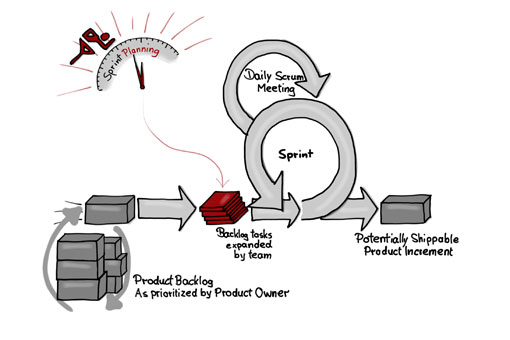
\includegraphics[width=\textwidth]{media/ProjectManagement/SprintPlanning.jpg}
    \caption{"Sprint Planning" Event \cite{PlanningBild}}
\end{figure}

In diesem Event werden sich einzelne Dinge aus dem "Product Backlog" herausgenommen, in das "Sprint Backlog" abgelegt und ein gewisses Ziel für das "Inkrement" festgelegt. \cite{Planning}

Die Dauer dieses Events ist unterschiedlich und kommt immer darauf an, wie lang der eigentliche "Sprint" angesetzt ist. Es kann jedoch gesagt werden, dass bei einem "Sprint", welcher über vier Wochen geht mit Acht Stunden für eine intensive Planung gerechnet werden kann. Teilnehmen tun an diesem Meeting alle Rollen im Scrum Projekt, also das Entwicklerteam, der "Scrum Master" und der "Product Owner". \cite{Planning}

"\underline{Daily Scrum}"

\begin{figure}[H]
    \centering
    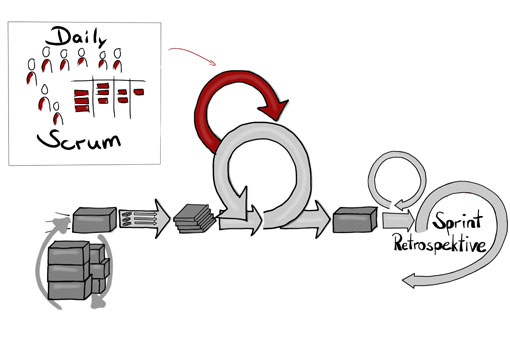
\includegraphics[width=\textwidth]{media/ProjectManagement/DailyScrum.jpg}
    \caption{"Daily Scrum" Event \cite{DailyScrumBild}}
\end{figure}

Das "Daily Scrum" findet jeden Tag statt und sollte im Optimalfall auch immer  zur gleichen Uhrzeit und am gleichen Ort abgehalten werden. Im "Scrum Guide" ist festgelegt, dass dieses tägliche Meeting nicht länger als 15 Minuten dauern sollte und nur dazu dienen die Teammitglieder auf den neuesten Stand zu bringen oder über Probleme zu informieren. "Daily Scrum" wird für gewöhnlich immer vom "Scrum Master" durchgeführt. Der "Scrum Master" kann jedoch auch jemanden aus dem Entwicklerteam darauf schulden das "Daily Scrum" abzuhalten um sich selbst mehr Zeitressourcen freizuhalten. \cite{DailyScrum}

In der Theorie gibt jede*r aus dem Entwicklerteam ein knappes Statement zu folgenden Fragen ab um das restliche Team über den Stand der Dinge zu informieren:

\begin{itemize}
    \item "Woran habe ich gestern gearbeitet, damit wir das Sprint-Ziel erreichen?" \cite{DailyScrum}
    \item "Womit möchte ich heute dazu beitragen, dass wir das Sprint-Ziel erreichen?" \cite{DailyScrum}
    \item "Was behindert mich oder das Entwicklungsteam daran, das Sprint-Ziel zu erreichen?" \cite{DailyScrum}
\end{itemize}

"\underline{Sprint}"

Der "Sprint" ist das elementare Stück bei "Scrum", da hier die tatsächliche Arbeit und Implementierung der Anforderungen im Projekt geschieht. Die Dauer eines "Sprints" kann in jedem Projekt unterschiedlich gehandhabt werden. Für gewöhnlich ist aber anzunehmen, dass sich die Dauer auf etwas zwischen Einer und vier Wochen beläuft. Eine längere Zeit für einen "Sprint" ist nicht explizit verboten, aber unüblich, da so eine gewisse Flexibilität verloren geht, welche in "Scrum" einen hohen Stellwert hat. \cite{Sprint}

Wie vorher schon erwähnt, werden in einem "Sprint" nun die einzelnen Anforderungen aus dem "Product Backlog" abgearbeitet. Sobald ein "Sprint" abgeschlossen ist, ist es wichtig, dass eine zum Teil funktionierende Software vorhanden ist um diese in das "Inkrement" zu verschieben. \cite{Sprint}

Im Vergleich mit klassischem Projektmanagement ist der "Sprint" als Ablaufplan zu verstehen, aber deutlich flexibler, da nur zwei Dinge im Vorhinein festgelegt werden müssen. Dies sind einerseits der Starttermin des Projekts und andererseits die Dauer eines "Sprints". Der Rest (Leistungsumfang) wird nun nur aus dem "Product Backlog" entnommen und zu Implementierung genutzt. \cite{Sprint}

"\underline{Sprint Review}"

In diesem Meeting werden vom Entwicklerteam die Ergebnisse des letzten "Sprints" genauer dargelegt und präsentiert. Es nehmen für gewöhnlich das Entwicklerteam, der "Scrum Master" und der "Product Owner" teil. Es kann aber auch vorkommen, dass der "Product Owner" manche Auftraggeber (Stakeholder) noch zusätzlich einlädt. Bei einer Sprintdauer von vier Woche kann ungefähr vier Stunden an "Reviewzeit" eingeplant werden. \cite{SprintReview}

Jedoch sind die unterschiedlichen Teilnehmer*innen für unterschiedliche Verantwortlichkeiten zuständig. Der "Scrum Master" ist für das einberufen des "Sprint Reviews" zuständig, während der "Product Owner" beschreiben muss, welcher der "User Stories" (Anforderungen, welche sich für dieses "Sprint" vorgenommen wurde) fertiggestellt wurde und welche nicht. Das Entwicklerteam stellt ihre erzielten Ergebnisse allen Meetingteilnehmer*innen vor. \cite{SprintReview}

Der Abschluss des "Sprint Reviews" wird durch eine gemeinsame Vorbereitung des nächsten "Sprint Plannings" gemacht. Dies geschieht unter Einbindung aller Teilnehmer*innen und unter Berücksichtigung zusätzlicher Faktoren (Budget oder Marktentwicklung), welche durch die Flexibilität bei "Scrum" sonst vielleicht zu kurz kommen würden. \cite{SprintReview}

"\underline{Sprint Retrospektive}"

In diesem Meeting nimmt nur das "Scrum Team" teil, also der "Scrum Master", der "Product Owner" und das Entwicklerteam. Auf die unterschiedlichen "Stakeholder" wird in dieser Besprechung verzichtet. Wenn ein Sprint vier Wochen gedauert hat ist es üblich, dass die Phase der Retrospektive drei Stunden dauert. Der "Scrum Master" übernimmt hierbei eine zentrale Rolle, da er das Meeting leitet und moderiert. Die Teilnehmer*innen bekommen für das drei Fragen gestellt um einen groben Überblick über das Arbeiten während des Sprints zu bekommen. \cite{SprintRetrospektive}

Die Leitfragen lauten wie folgt:

\begin{itemize}
    \item "Welche positiven und negativen Erfahrungen haben wir im vergangenen Sprint gemacht?" \cite{SprintRetrospektive}
    \item "Was wollen wir verbessern?" \cite{SprintRetrospektive}
    \item "Wie setzen wir diese Verbesserungen um?" \cite{SprintRetrospektive}
\end{itemize}
